%\documentclass[handout,xcolor=pdftex,dvipsnames,table]{beamer}
%\documentclass[draft]{beamer}
%\documentclass[notesonly]{beamer}
%\documentclass[notes]{beamer}
\documentclass[aspectratio=169, xcolor=table]{beamer}\usepackage[]{graphicx}\usepackage[]{color}
%% maxwidth is the original width if it is less than linewidth
%% otherwise use linewidth (to make sure the graphics do not exceed the margin)
\makeatletter
\def\maxwidth{ %
  \ifdim\Gin@nat@width>\linewidth
    \linewidth
  \else
    \Gin@nat@width
  \fi
}
\makeatother

\definecolor{fgcolor}{rgb}{0.345, 0.345, 0.345}
\newcommand{\hlnum}[1]{\textcolor[rgb]{0.686,0.059,0.569}{#1}}%
\newcommand{\hlstr}[1]{\textcolor[rgb]{0.192,0.494,0.8}{#1}}%
\newcommand{\hlcom}[1]{\textcolor[rgb]{0.678,0.584,0.686}{\textit{#1}}}%
\newcommand{\hlopt}[1]{\textcolor[rgb]{0,0,0}{#1}}%
\newcommand{\hlstd}[1]{\textcolor[rgb]{0.345,0.345,0.345}{#1}}%
\newcommand{\hlkwa}[1]{\textcolor[rgb]{0.161,0.373,0.58}{\textbf{#1}}}%
\newcommand{\hlkwb}[1]{\textcolor[rgb]{0.69,0.353,0.396}{#1}}%
\newcommand{\hlkwc}[1]{\textcolor[rgb]{0.333,0.667,0.333}{#1}}%
\newcommand{\hlkwd}[1]{\textcolor[rgb]{0.737,0.353,0.396}{\textbf{#1}}}%
\let\hlipl\hlkwb

\usepackage{framed}
\makeatletter
\newenvironment{kframe}{%
 \def\at@end@of@kframe{}%
 \ifinner\ifhmode%
  \def\at@end@of@kframe{\end{minipage}}%
  \begin{minipage}{\columnwidth}%
 \fi\fi%
 \def\FrameCommand##1{\hskip\@totalleftmargin \hskip-\fboxsep
 \colorbox{shadecolor}{##1}\hskip-\fboxsep
     % There is no \\@totalrightmargin, so:
     \hskip-\linewidth \hskip-\@totalleftmargin \hskip\columnwidth}%
 \MakeFramed {\advance\hsize-\width
   \@totalleftmargin\z@ \linewidth\hsize
   \@setminipage}}%
 {\par\unskip\endMakeFramed%
 \at@end@of@kframe}
\makeatother

\definecolor{shadecolor}{rgb}{.97, .97, .97}
\definecolor{messagecolor}{rgb}{0, 0, 0}
\definecolor{warningcolor}{rgb}{1, 0, 1}
\definecolor{errorcolor}{rgb}{1, 0, 0}
\newenvironment{knitrout}{}{} % an empty environment to be redefined in TeX

\usepackage{alltt}  % xcolor to avoid conflict
                                                       %  with beamer
\mode<presentation>
% https://hartwork.org/beamer-theme-matrix/
\usetheme{Singapore} %Berkeley, Palo Alto, Singapore, Warsaw
\usecolortheme{seahorse}  %Beaver, dolphin, dove, lily, orchid, seagull, seahorse
\renewcommand{\insertnavigation}[1]{}    % to remove contents bar:
           % https://tex.stackexchange.com/questions/33767/remove-section-header-from-a-beamer-theme-singapore

%\usefonttheme{serif}
% font themes: default, professionalfonts, serif, structurebold, structureitalicserif, structuresmallcapsserif

\usepackage{graphicx}
\usepackage{pgf}
\usepackage{array}
\usepackage{tabularx}
\usepackage{multicol}          %% Multiple columns for itemize
%\usepackage{booktabs}          %% Used in risk tables [hake]
%\usepackage{multirow}          %% Used in decision tables [hake]
%\usepackage{beamerarticle}
%\usepackage{enumitem}
%\usepackage{beamerthemesplit}
\usepackage[T1]{fontenc}  %to use < or > in tables
% \usepackage{xcolor}            %% for kable
% \usepackage[table]{xcolor}            %% for kable

% From kableExtra documentation, commenting out some:
\usepackage{longtable}
\usepackage{array}
\usepackage[table]{xcolor}
\usepackage{booktabs}          %% Used in risk tables [hake]
\usepackage{multirow}          %% Used in decision tables [hake]

\usepackage{wrapfig}
\usepackage{float}
\usepackage{colortbl}
\usepackage{pdflscape}
\usepackage{tabu}
\usepackage{threeparttable}
\usepackage{threeparttablex}
\usepackage[normalem]{ulem}
\usepackage{makecell}

\usepackage[export]{adjustbox}     % for left and right in \includegraphics
\usepackage[absolute,overlay]{textpos}  % for overlaying text

\newcolumntype{Y}{>{\centering\arraybackslash}X}
%% syntax is \mlc{first line\\secondline}
\newcommand{\mlc}[2][c]{\begin{tabular}[#1]{@{}c@{}}#2\end{tabular}}
\newcommand{\subscr}[1]{$_{\text{#1}}$}\newcommand{\Fforty}{F_{\text{SPR}=40\%}}       % Needs to be done as $\Fforty$
\newcommand{\Bforty}{B_{\text{SPR}=40\%}}

% pdf is displayed in full screen mode automatically
%\hypersetup{pdfpagemode=FullScreen}

%\setbeamersize{sidebar width left=0.05in}
\setbeamersize{text margin left=5mm}
\setbeamersize{text margin right=5mm}

\setbeamertemplate{title page}
{
% Looks like for hake we didn't use the defaults and played with the spacing
% \vskip0pt plus 1filll
\begin{center}
\vskip6pt
{\usebeamerfont{title}\usebeamercolor[fg]{title}\inserttitle}\\
\vskip22pt
\insertauthor
\vskip22pt
\insertinstitute
% \insertdate
\end{center}
% \vskip30pt
\vfill
\usebeamerfont{subtitle}\usebeamercolor[fg]{subtitle}\insertsubtitle % \par
% \vskip0pt plus 1filll
\hfill

\includegraphics[width=4.8cm]{images/DFO_Logo.png}   % from Wikipedia (for hake we
% had an older one)
\includegraphics[width=1cm]{images/UBC-logo.jpg}
\vskip10pt
}

\definecolor{pageCol}{rgb}{0.5,0.5,1.0}

\setbeamertemplate{footline}
{
\begin{beamercolorbox}[wd=.05\paperwidth,ht=0ex,dp=0ex,left]{framenumber in head/foot}%
\insertframenumber/\inserttotalframenumber
\end{beamercolorbox}%
}
%% \setbeamercolor{footline}{fg=pageCol}

\newcounter{saveenumi}

\newcommand{\blue}{\textcolor{blue}}
\newcommand{\red}{\textcolor{red}}
\newcommand{\bc}{\begin{center}}
\newcommand{\ec}{\end{center}}
\newcommand{\bn}{\begin{enumerate}}
\newcommand{\en}{\end{enumerate}}
\newcommand{\bi}{\begin{itemize}}
\newcommand{\ei}{\end{itemize}}
\newcommand{\Bmsy}{B_{\mbox{\tiny{MSY}}}}
\newcommand{\howlikely}{How likely are different values of $p$ (the underlying probability of getting a head)?}
%% <<echo=TRUE,  message=TRUE, results='show', warning=TRUE>>=
%% opts_chunk$set(dev='cairo_ps',fig.path='knitr-cache/', fig.dpi=96, fig.width=7.5,
%%                fig.height=4, echo=TRUE, results=TRUE, message=TRUE, warning=TRUE,
%%                results='show', cache=TRUE, cache.path='knitr-cache/')


%%%%%%%%%%%%%%%%%%%%%%%%%%%%%%%%%%%%%%%%%%%%%%%%%%%%%%%%%%%%%%%%%


\title[Notation]{~\\ Some guidance on using mathematical notation in biology}
\author{Andrew Edwards\\ ~\\ 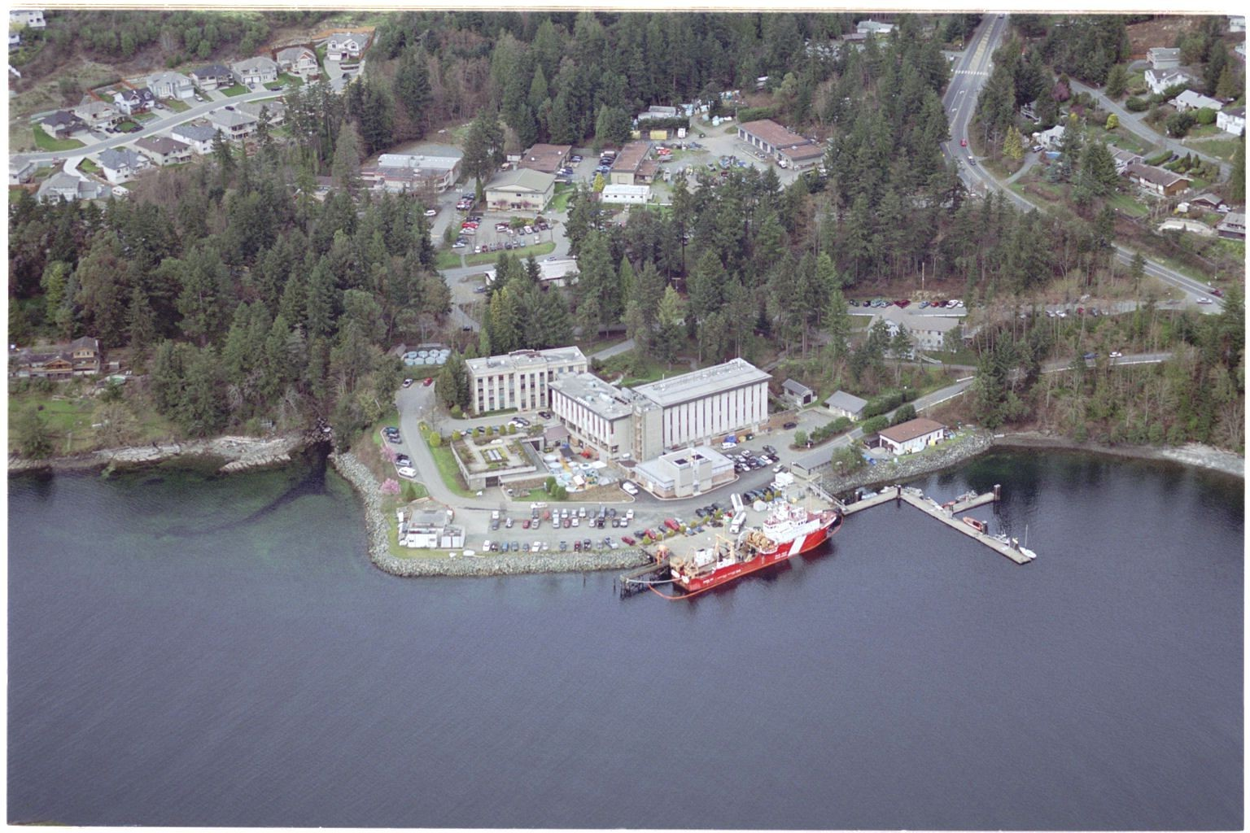
\includegraphics[height=3.5cm]{images/pbs.png}\\
  ~\\ \textcolor{blue}{Pacific Biological Station \& University of Victoria}}
% \institute{{\textcolor{blue}{Pacific Biological Station, Nanaimo, BC}\\
%  ~\\
% \institute{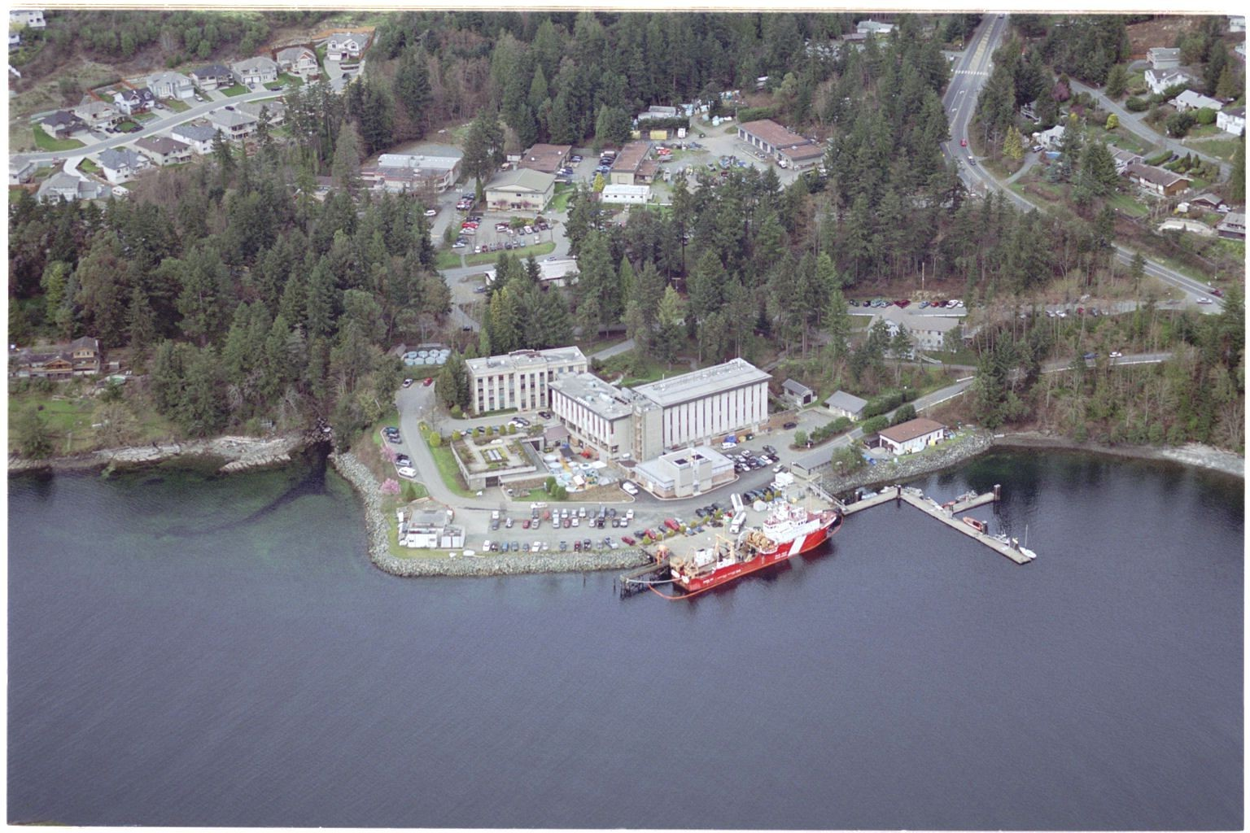
\includegraphics[height=3cm]{images/pbs.png}}
% \titlegraphic{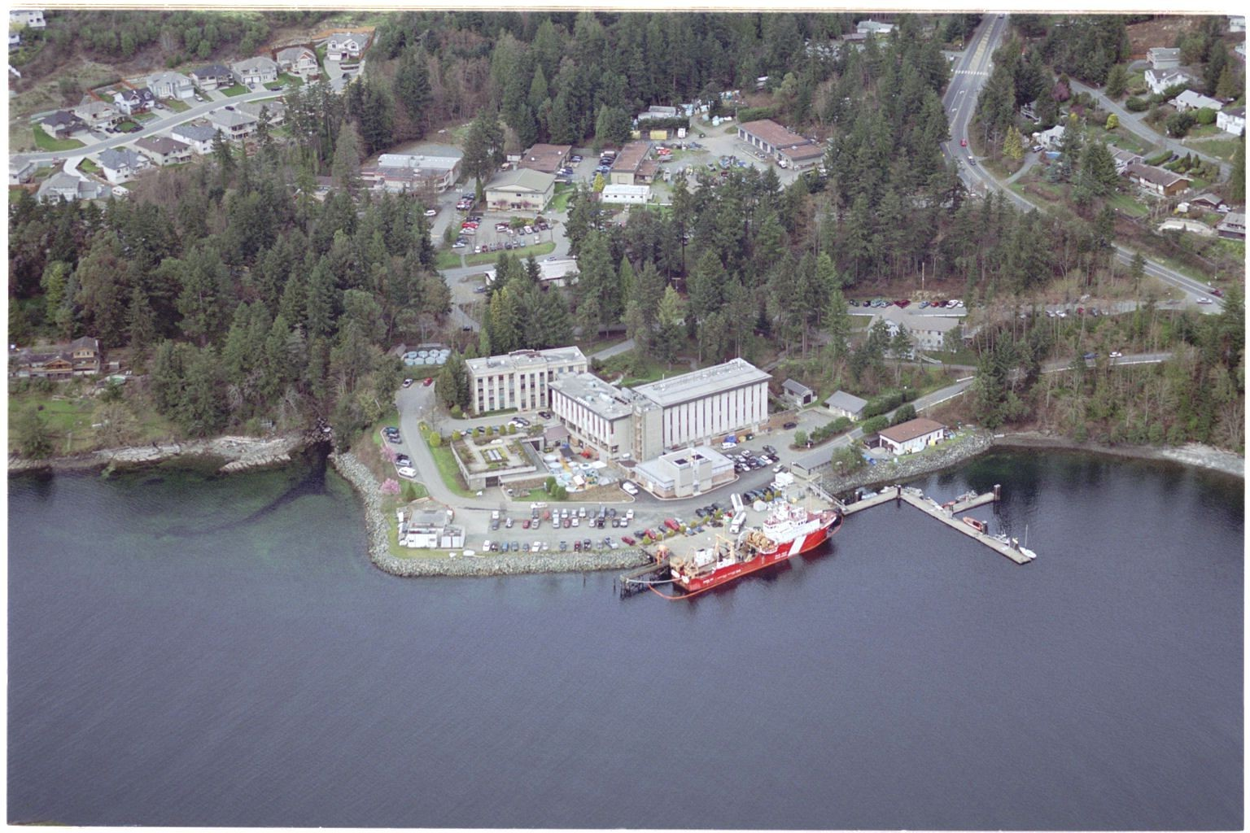
\includegraphics[height=3.3cm]{images/pbs.png}}
% \titlegraphic{images/pbs.png}
\date{{\footnotesize SRG meeting -- 2018}}
\subtitle{\small UVic Biology Department Seminar\\
Friday 1st November, 2019}
\IfFileExists{upquote.sty}{\usepackage{upquote}}{}

\setbeamertemplate{background}
{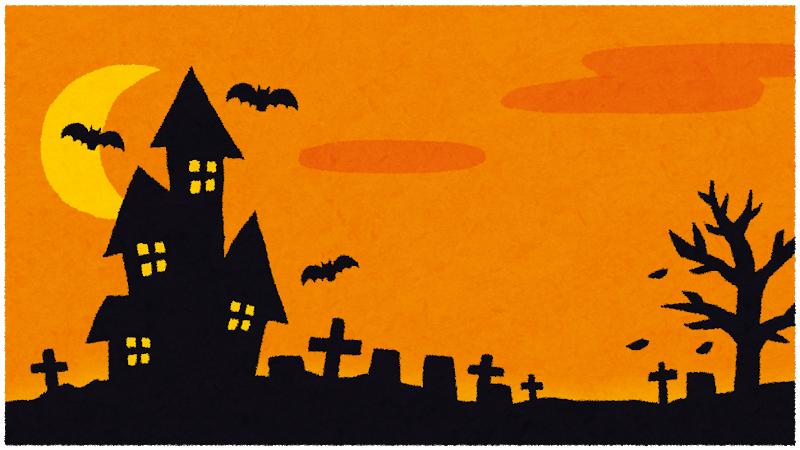
\includegraphics[width=\paperwidth,height=\paperheight,keepaspectratio]{images/halloween_background_orange.png}}

\begin{document}

\beamertemplatenavigationsymbolsempty   % bottom navigation panel
% \setbeamertemplate{headline}{}
% \setbeamertemplate{mini frames}{}

%\begin[plain]{frame}
\frame[plain]{
\titlepage
}
%----------------------------------------------------------

\end{document}

\begin{frame}
\frametitle{Aims of this lecture}
% ~\\

I hope that you'll come away with an understanding of:

~\\

\begin{minipage}{12cm}
\bi
  \item how stock assessment scientists can include
    uncertainty in advice to managers
  \item \textcolor{blue}{how to interpret such uncertainty}
  % \item The concepts behind these Relate the concepts to fairly simple examples
  \item some of the methods used to quantify uncertainty
  \item \textcolor{blue}{caveats and potential pitfalls}
\ei
\end{minipage}
\end{frame}



%%%%%%%%%%%%%%%%%%%%%%%
\section{Outline}
\subsection{}
\frame{\frametitle{Outline}
\bi
  \item Basic introduction to probability
  \item Examples of probabilities that we can calculate in assessments
  \item Presenting uncertainty in assessments
  \bi
    \item Stock status
    \item Projections
    \item Decision tables
  \ei
  \item Brief details of how probabilities get calculated
  \bi
    \item Likelihood
    \item Bayesian analysis
  \ei
  \item Other sources of uncertainty -- big caveat
  \item Risk
  \item Concluding remarks
\ei
}


%----------------------------------------------------------

\begin{frame}
\frametitle{About me}
~\\

\begin{minipage}{12cm}
\bi
  \item Pacific Biological Station since 2007
  \item Previously at Bedford Institute of Oceanography \& Dalhousie
\ei
\end{minipage}
\begin{minipage}{2cm}
  \includegraphics[width=1.3cm, right]{images/andyCrop2.jpg}
\end{minipage}

\bi
  \item Stock assessment work:
    \bi
    \item rockfish (long-lived, good age data)
    \item Pacific Hake (joint with U.S. colleagues)
    \item data synopsis for $>100$ species of British Columbia groundfish
  \ei
  \item Recent research:
  \bi
    \item methods for fitting size spectra
    \item notation guidelines (in press):
  \ei
\ei
\medskip
%\hfill
\pause
% \includegraphics[width=5cm, right]{images/MEE.png}\\
~~~\includegraphics[width=10cm, center]{images/notation-header.png}
% \vskip10pt
\end{frame}

% ----------------------------------------------------------

\begin{frame}
\frametitle{Example of data (Pacific Hake)}

% \centering

\begin{minipage}{8cm}
\includegraphics[height=6cm]{images/hake-ages.png}
\end{minipage}
\begin{minipage}{5cm}
~~~~~~~~~~~~~~~~~~~~\includegraphics[height=1.5cm, right]{images/hake-pic.png}
\end{minipage}

\end{frame}

%----------------------------------------------------------

\begin{frame}
\frametitle{What is the probability that the stock is in the healthy zone?}

\centering
\includegraphics[height=2.5in]{images/PA-graph.png}

\end{frame}

% ----------------------------------------------------------

\begin{frame}
\frametitle{Schematic of a model (Pacific Ocean Perch)}

\centering
\includegraphics[height=4in]{images/model-schematic.png}

\end{frame}

% ----------------------------------------------------------

%%%%%%%%%%%%%%%%%%%%%%%
\section{Introduction to probability}
\subsection{}

\begin{frame}
\frametitle{Introduction to probability}

\includegraphics[height=1.5cm, right]{images/coin-toss.png}

\begin{tabular}{lrrrr}
  & Fraction & Decimal & Percentage & Odds \\
  & & & & \\
Probability that a tossed coin lands heads: & $\dfrac{1}{2}$ & \alert<3-4>{0.5} &
  \textcolor<4>{blue}{50\%} & \textcolor<4>{blue}{1 in 2} \\
  & & & & \\
\onslide<2->Probability that a rolled die gives a six: & $\dfrac{1}{6}$ &
  \alert<3-4>{0.167} & \textcolor<4>{blue}{16.7\%} & \textcolor<4>{blue}{1 in 6}
\end{tabular}
\includegraphics<2-4>[height=1cm, right]{images/die-roll.png}

% \begin{minipage}{8cm}
\onslide<3-4>\alert{~~Easier to use in calculations}
\onslide<4>\rightline{\textcolor{blue}{May be more easily understood by stakeholders}}
% end{minipage}

%\begin{minipage}{1.5cm}
% \includegraphics<2-4>[height=1.5cm, right]{images/die-roll.png}
%
% \end{minipage}

\end{frame}

%----------------------------------------------------------

\begin{frame}
\frametitle{Introduction to probability}

Probability is always of \alert{\emph{some event happening}}, for example:

\bi
\item probability that \alert{\emph{a tossed coin lands heads}}
\ei

Write this as:

\bi
\item P(a tossed coin lands heads)
\item P(heads)
\ei

\pause

~\\

Other events:
\bi
\item P(a die roll gives a 6)
\item P(fish stock is currently in the healthy zone)
\ei

\end{frame}

%----------------------------------------------------------

\begin{frame}
\frametitle{Introduction to probability}

\begin{tabular}{ll}
  & \\
Values of probabilities  & Examples \\
  \hline
P(impossible event) = 0 & \textcolor{blue}{P(standard die gives a 7)} \\
  & \\
P(definite event) = 1 & \textcolor{blue}{P(everyone's children got too much candy}\\
  &                     \textcolor{blue}{~~~~trick-or-treating last night)} \\
  & \\
Everything else is between 0 and 1 & \textcolor{blue}{P(it will rain tomorrow at a given location)}\\
                                   & \textcolor{blue}{P(fish stock is currently in the healthy zone)}
\end{tabular}

\pause

~\\

~\\

Probabilities of \textcolor{red}{all possible events} add up to 1:
\begin{eqnarray}
\nonumber \mbox{P(heads)} & = & 0.5\\
\nonumber \mbox{P(tails)} & = & 0.5\\
\nonumber \mbox{P(heads)} + \mbox{P(tails)} & = & 1
\end{eqnarray}
\end{frame}
%                            (the coin must lands on heads or tails)
%----------------------------------------------------------

\begin{frame}
\frametitle{Discrete outcomes}

A die roll can only produce \alert{discrete} values: 1, 2, 3, 4, 5 or 6.

~\\

Roll it 600 times and count up number from each roll:

~\\
\begin{knitrout}
\definecolor{shadecolor}{rgb}{0.969, 0.969, 0.969}\color{fgcolor}
\includegraphics[width=\maxwidth]{knitr-cache/roll-1}

\end{knitrout}

\end{frame}

%----------------------------------------------------------

%\begin{frame}
%\frametitle{Discrete outcomes}
%
%Similarly, count data are \alert{discrete} and take whole numbers.
%
%~\\
%
%Such as annual numbers of lynx trappings for 1821-1934 in Canada:
%
%~\\
%
%~~269,  321,  585,  871, 1475, 2821, 3928, 5943, 4950, 2577, 523, ...
%
% lynx[1:11]
%~\\
%
%Take those first 11 years and sort into order:
%
% sort(lynx[1:11])
%~\\
%
%~~269  321  523 585  871 \alert<2->{1475} 2577 2821 3928 4950 5943
%
%\\
%
%onslide<2-> \alert{Median} is the value in the middle
%
%\onslide<3-> \textcolor{blue}{Mean} is 2205.7, the total divided by 11.
%
%\end{frame}
%----------------------------------------------------------

\begin{frame}
\frametitle{Continuous data}

% hist(lynx, breaks=30)
% hist(lynx, breaks=100)

But many measured values are \alert{continuous} -- they can take any value from
a continuous range. For example:

\bi
\item weight
\item length
\item temperature
\item depth
\ei

To plot we have to bin the data, e.g. weights of 500 fish:

\begin{knitrout}
\definecolor{shadecolor}{rgb}{0.969, 0.969, 0.969}\color{fgcolor}
\includegraphics[width=\maxwidth]{knitr-cache/hist-simp-1}

\end{knitrout}




\end{frame}
%----------------------------------------------------------

\begin{frame}
\frametitle{Continuous variables}

To calculate probabilities, would first involve fitting a model:

\begin{knitrout}
\definecolor{shadecolor}{rgb}{0.969, 0.969, 0.969}\color{fgcolor}
\includegraphics[width=\maxwidth]{knitr-cache/hist-simp-2-1}

\end{knitrout}

\end{frame}

%----------------------------------------------------------

\begin{frame}
\frametitle{Continuous variables}

Now we have a model, we can ask questions:

~\\

\begin{knitrout}
\definecolor{shadecolor}{rgb}{0.969, 0.969, 0.969}\color{fgcolor}
\includegraphics[width=\maxwidth]{knitr-cache/hist-simp-3-1}

\end{knitrout}

What is the probability that a random fish weighs $>$120~g?

~\\

~\\

\end{frame}


%----------------------------------------------------------

\begin{frame}
\frametitle{Continuous variables}

Now we have a model, we can ask questions:

~\\

\begin{knitrout}
\definecolor{shadecolor}{rgb}{0.969, 0.969, 0.969}\color{fgcolor}
\includegraphics[width=\maxwidth]{knitr-cache/hist-simp-4-1}

\end{knitrout}

What is the probability that a random fish weighs $>$120~g?

~\\

P(fish weight $>$120~g) is the \textcolor{blue}{area shaded in blue}.


\end{frame}


%----------------------------------------------------------

\begin{frame}
\frametitle{Continuous variables}

Now we have a model, we can ask questions:

~\\

\begin{knitrout}
\definecolor{shadecolor}{rgb}{0.969, 0.969, 0.969}\color{fgcolor}
\includegraphics[width=\maxwidth]{knitr-cache/hist-simp-5-1}

\end{knitrout}

Similarly, what is probability of random fish weighing between 75 and 85~g?

P(75 $<$ fish weight $<$ 85) is the \textcolor{blue}{area shaded in blue}.

~\\

Since weight is continuous, we cannot ask P(fish weight = 120~g).

\end{frame}


%----------------------------------------------------------

\begin{frame}
\frametitle{Key terms}

For any distribution, we can give:

~\\

\begin{knitrout}
\definecolor{shadecolor}{rgb}{0.969, 0.969, 0.969}\color{fgcolor}
\includegraphics[width=\maxwidth]{knitr-cache/hist-simp-7-1}

\end{knitrout}

\textcolor{blue}{Median}. P(being $<$ median) = 0.5

~\\

\end{frame}


%----------------------------------------------------------

\begin{frame}
\frametitle{Key terms}

And various other values:

~\\

\begin{knitrout}
\definecolor{shadecolor}{rgb}{0.969, 0.969, 0.969}\color{fgcolor}
\includegraphics[width=\maxwidth]{knitr-cache/hist-simp-8-1}

\end{knitrout}

\textcolor{blue}{2.5\% percentile}. P(being $<$ this value) = 0.025
% ~~[2.5\% of the values lie beneath this value]

~\\

\end{frame}

% ----------------------------------------------------------

\begin{frame}
\frametitle{Key terms}

One way of summarising resulting distributions is through boxplots:

~\\

\begin{knitrout}
\definecolor{shadecolor}{rgb}{0.969, 0.969, 0.969}\color{fgcolor}
\includegraphics[width=\maxwidth]{knitr-cache/hist-simp-9-1}

\end{knitrout}
\textcolor{blue}{Median 50\% percentile}  % -- P(being $<$ this value) = 0.025

~\\

\end{frame}

%----------------------------------------------------------


\begin{frame}
\frametitle{Key terms}

One way of summarising resulting distributions is through boxplots:

~\\

\begin{knitrout}
\definecolor{shadecolor}{rgb}{0.969, 0.969, 0.969}\color{fgcolor}
\includegraphics[width=\maxwidth]{knitr-cache/hist-simp-12-1}

\end{knitrout}
\textcolor{blue}{2.5\% percentile}  % -- P(being $<$ this value) = 0.025

~\\

\end{frame}

% ------------------------------------------------

\begin{frame}
\frametitle{Key terms}

One way of summarising resulting distributions is through boxplots:

~\\

\begin{knitrout}
\definecolor{shadecolor}{rgb}{0.969, 0.969, 0.969}\color{fgcolor}
\includegraphics[width=\maxwidth]{knitr-cache/hist-simp-13-1}

\end{knitrout}
\textcolor{blue}{25\% percentile}  % -- P(being $<$ this value) = 0.025

~\\

\end{frame}

% ------------------------------------------------

\begin{frame}
\frametitle{Key terms}

One way of summarising resulting distributions is through boxplots:

~\\

\begin{knitrout}
\definecolor{shadecolor}{rgb}{0.969, 0.969, 0.969}\color{fgcolor}
\includegraphics[width=\maxwidth]{knitr-cache/hist-simp-10-1}

\end{knitrout}
\textcolor{blue}{75\% percentile}  % -- P(being $<$ this value) = 0.025

~\\

\end{frame}

% ----------------------------------------------------------

\begin{frame}
\frametitle{Key terms}

One way of summarising resulting distributions is through boxplots:

~\\

\begin{knitrout}
\definecolor{shadecolor}{rgb}{0.969, 0.969, 0.969}\color{fgcolor}
\includegraphics[width=\maxwidth]{knitr-cache/hist-simp-11-1}

\end{knitrout}
\textcolor{blue}{97.5\% percentile}  % -- P(being $<$ this value) = 0.025

~\\

\end{frame}

% ----------------------------------------------------------

\begin{frame}
\frametitle{Communicating uncertainty}

Catch data and vulnerable biomass estimated from a model:

\centering
\includegraphics[height=2in]{images/quantiles.png}
~~~~~
\includegraphics[height=2.5in]{images/vulnerable.png}

\end{frame}

%----------------------------------------------------------

\begin{frame}
\frametitle{Communicating uncertainty}

Estimated recruitment (1000's of age-1 individuals) through time:

\centering
\includegraphics[height=2.5in]{images/recruitment.png}

\end{frame}

%----------------------------------------------------------

\begin{frame}
\frametitle{Results in context of precautionary-approach figure}

\centering
\includegraphics[height=2.5in]{images/PA-graph.png}

\end{frame}

%----------------------------------------------------------

\begin{frame}
\frametitle{Results in context of precautionary-approach figure}

\centering
\includegraphics[height=2.5in]{images/POP-status.png}

\end{frame}

%----------------------------------------------------------

\begin{frame}
\frametitle{Results in context of precautionary-approach figure}

\centering
\includegraphics[height=2.5in]{images/POP-status2.png}

\end{frame}

%----------------------------------------------------------

\begin{frame}
\frametitle{Results in context of precautionary-approach figure}

\centering
\includegraphics[height=2.5in]{images/snail-2.png}

Here it would be too much to show uncertainty for \alert{all} years.

\end{frame}

% ----------------------------------------------------------

\begin{frame}

\frametitle{Questions?}

Any question so far?

\pause

~\\

~\\

\includegraphics[width=8cm, center]{images/correlation.png}

\end{frame}

% ----------------------------------------------------------

\begin{frame}
\frametitle{Going forward -- projections}

\bc
Historical and projected spawning biomass

~\\

\includegraphics[height=14cm]{images/projections-crop.png}
\ec

\end{frame}

%----------------------------------------------------------


\begin{frame}
\frametitle{Going forward -- projections}

\begin{minipage}{4cm}
Historical and projected spawning biomass for various catch levels
\end{minipage}
\begin{minipage}{10cm}
\includegraphics[height=7.5cm]{images/projections.png}
\end{minipage}

\end{frame}

%----------------------------------------------------------

\begin{frame}
\frametitle{Decision tables}

\centering P($B_t > 0.8 \Bmsy)$, i.e.~stock in healthy zone at start of year $t$
\begin{table}[H]
\centering\rowcolors{2}{gray!6}{white}

\begin{tabular}{>{\raggedleft\arraybackslash}p{2.5cm}rrrrrr}
\hiderowcolors
\toprule
Annual catch strategy (t) & 2013 & 2014 & 2015 & 2016 & 2017 & 2018\\
\midrule
\showrowcolors
0 & 0.87 & 0.88 & 0.90 & 0.92 & 0.93 & 0.94\\
200 & 0.87 & 0.88 & 0.89 & 0.90 & 0.91 & 0.92\\
400 & 0.87 & 0.87 & 0.88 & 0.88 & 0.89 & 0.90\\
600 & 0.87 & 0.86 & 0.86 & 0.86 & 0.87 & 0.87\\
800 & 0.87 & 0.86 & 0.85 & 0.85 & 0.85 & 0.85\\
1000 & 0.87 & 0.85 & 0.83 & 0.83 & 0.82 & 0.81\\
\bottomrule
\end{tabular}
\rowcolors{2}{white}{white}
\end{table}



~\\
% 600 t is just above average recent catch of 547 t

\end{frame}

\begin{frame}
\frametitle{Decision tables}

\centering P($B_t > 0.8 \Bmsy)$, i.e.~stock in healthy zone at start of year $t$
\begin{table}[H]
\centering\rowcolors{2}{gray!6}{white}

\begin{tabular}{>{\raggedleft\arraybackslash}p{2.5cm}rrrrrr}
\hiderowcolors
\toprule
Annual catch strategy (t) & 2013 & 2014 & 2015 & 2016 & 2017 & 2018\\
\midrule
\showrowcolors
\textcolor{red}{0} & \textcolor{red}{0.87} & \textcolor{red}{0.88} & \textcolor{red}{0.90} & \textcolor{red}{0.92} & \textcolor{red}{0.93} & \textcolor{red}{0.94}\\
200 & 0.87 & 0.88 & 0.89 & 0.90 & 0.91 & 0.92\\
400 & 0.87 & 0.87 & 0.88 & 0.88 & 0.89 & 0.90\\
600 & 0.87 & 0.86 & 0.86 & 0.86 & 0.87 & 0.87\\
800 & 0.87 & 0.86 & 0.85 & 0.85 & 0.85 & 0.85\\
1000 & 0.87 & 0.85 & 0.83 & 0.83 & 0.82 & 0.81\\
\bottomrule
\end{tabular}
\rowcolors{2}{white}{white}
\end{table}



~\\

% 600 t is just above average recent catch of 547 t

\end{frame}


%----------------------------------------------------------

\begin{frame}
\frametitle{Decision tables}

\centering P($B_t > 0.8 \Bmsy)$, i.e.~stock in healthy zone at start of year $t$
\begin{table}[H]
\centering\rowcolors{2}{gray!6}{white}

\begin{tabular}{>{\raggedleft\arraybackslash}p{2.5cm}rrrrrr}
\hiderowcolors
\toprule
Annual catch strategy (t) & 2013 & 2014 & 2015 & 2016 & 2017 & 2018\\
\midrule
\showrowcolors
0 & 0.87 & 0.88 & 0.90 & 0.92 & 0.93 & 0.94\\
200 & 0.87 & 0.88 & 0.89 & 0.90 & 0.91 & 0.92\\
400 & 0.87 & 0.87 & 0.88 & 0.88 & 0.89 & 0.90\\
\textcolor{red}{600} & \textcolor{red}{0.87} & \textcolor{red}{0.86} & \textcolor{red}{0.86} & \textcolor{red}{0.86} & \textcolor{red}{0.87} & \textcolor{red}{0.87}\\
800 & 0.87 & 0.86 & 0.85 & 0.85 & 0.85 & 0.85\\
1000 & 0.87 & 0.85 & 0.83 & 0.83 & 0.82 & 0.81\\
\bottomrule
\end{tabular}
\rowcolors{2}{white}{white}
\end{table}



~\\
% 600 t is just above average recent catch of 547 t

\end{frame}


%----------------------------------------------------------

\begin{frame}
\frametitle{Decision tables}

\centering P($B_t > 0.8 \Bmsy)$, i.e.~stock in healthy zone at start of year $t$
\begin{table}[H]
\centering\rowcolors{2}{gray!6}{white}

\begin{tabular}{>{\raggedleft\arraybackslash}p{2.5cm}rrrrrr}
\hiderowcolors
\toprule
Annual catch strategy (t) & 2013 & 2014 & 2015 & 2016 & 2017 & 2018\\
\midrule
\showrowcolors
0 & 0.87 & 0.88 & 0.90 & 0.92 & 0.93 & 0.94\\
200 & 0.87 & 0.88 & 0.89 & 0.90 & 0.91 & 0.92\\
400 & 0.87 & 0.87 & 0.88 & 0.88 & 0.89 & 0.90\\
600 & 0.87 & 0.86 & 0.86 & 0.86 & 0.87 & 0.87\\
800 & 0.87 & 0.86 & 0.85 & 0.85 & 0.85 & 0.85\\
\textcolor{red}{1000} & \textcolor{red}{0.87} & \textcolor{red}{0.85} & \textcolor{red}{0.83} & \textcolor{red}{0.83} & \textcolor{red}{0.82} & \textcolor{red}{0.81}\\
\bottomrule
\end{tabular}
\rowcolors{2}{white}{white}
\end{table}



~\\

\end{frame}


% ----------------------------------------------------------


\begin{frame}
\frametitle{Fisheries manager had another interpretation}

\centering P($B_t > 0.8 \Bmsy)$, i.e.~stock in healthy zone at start of year $t$
\begin{table}[H]
\centering\rowcolors{2}{gray!6}{white}

\begin{tabular}{>{\raggedleft\arraybackslash}p{2.5cm}rr>{\leavevmode\color{red}}rrrr}
\hiderowcolors
\toprule
Annual catch strategy (t) & 2013 & 2014 & 2015 & 2016 & 2017 & 2018\\
\midrule
\showrowcolors
0 & 0.87 & 0.88 & 0.90 & 0.92 & 0.93 & 0.94\\
200 & 0.87 & 0.88 & 0.89 & 0.90 & 0.91 & 0.92\\
400 & 0.87 & 0.87 & 0.88 & 0.88 & 0.89 & 0.90\\
600 & 0.87 & 0.86 & 0.86 & 0.86 & 0.87 & 0.87\\
800 & 0.87 & 0.86 & 0.85 & 0.85 & 0.85 & 0.85\\
1000 & 0.87 & 0.85 & 0.83 & 0.83 & 0.82 & 0.81\\
\bottomrule
\end{tabular}
\rowcolors{2}{white}{white}
\end{table}



~\\

\end{frame}

% ----------------------------------------------------------

\begin{frame}

\frametitle{What if results had been the other way around?}

\centering P($B_t$\alert{$\leq$} $0.8 \Bmsy)$, i.e.~stock is \alert{below} healthy zone at start of year $t$
\begin{table}[H]
\centering\rowcolors{2}{gray!6}{white}

\begin{tabular}{>{\raggedleft\arraybackslash}p{2.5cm}rr>{\leavevmode\color{red}}rrrr}
\hiderowcolors
\toprule
Annual catch strategy (t) & 2013 & 2014 & 2015 & 2016 & 2017 & 2018\\
\midrule
\showrowcolors
0 & 0.13 & 0.12 & 0.10 & 0.08 & 0.07 & 0.06\\
200 & 0.13 & 0.12 & 0.11 & 0.10 & 0.09 & 0.08\\
400 & 0.13 & 0.13 & 0.12 & 0.12 & 0.11 & 0.10\\
600 & 0.13 & 0.14 & 0.14 & 0.14 & 0.13 & 0.13\\
800 & 0.13 & 0.14 & 0.15 & 0.15 & 0.15 & 0.15\\
1000 & 0.13 & 0.15 & 0.17 & 0.17 & 0.18 & 0.19\\
\bottomrule
\end{tabular}
\rowcolors{2}{white}{white}
\end{table}



~\\


\end{frame}

%----------------------------------------------------------

\begin{frame}
\frametitle{Decision tables}

For Pacific Ocean Perch assessments we have tended to give P(in healthy zone) etc.,

~~i.e. probability of being in a good place (glass half-full).

~\\

Other assessments tend to show P(being in bad place), e.g. P(below healthy zone).


\end{frame}
%----------------------------------------------------------

\begin{frame}
\frametitle{Pacific Hake -- other way round}

Pacific Hake (different type of table -- shows various probabilities
under different catches for just one year):

\centering
\includegraphics[height=7.5cm]{images/hake-dec-table.png}

\end{frame}

% ----------------------------------------------------------

\begin{frame}
\frametitle{Beware!!}

So be aware and double check definitions in the tables!

~\\

No general rule as to which way to do them.

~\\

Often historical legacy, so can be confusing to change for a particular species
to create consistency.

~\\

In fisheries science, a decision table presents \alert{potential consequences of different decisions},\\
and is used to help facilitate decision making.

\end{frame}

% ----------------------------------------------------------

\begin{frame}
\frametitle{Beware!!}

Note also the representation of probabilities as \% rather than decimals.

Was originally preferred by stakeholders.

\centering
\includegraphics[height=7.5cm]{images/hake-dec-table.png}


\end{frame}

% ----------------------------------------------------------

\begin{frame}
\frametitle{How could fisheries managers use information to make decisions?}

\centering
\includegraphics[height=7.5cm]{images/combine-results.png}

\end{frame}

% ----------------------------------------------------------

\begin{frame}
\frametitle{So how do we obtain these probabilities?}

\centering
\includegraphics[height=4in]{images/model-schematic.png}

\end{frame}

% --------------------------------------

\begin{frame}
\frametitle{So how do we obtain these probabilities?}

Helpful to understand the ideas behind calculating these
probabilities
(and why people in assessment review meetings spend so much time
talking about those damn `priors').

~\\

Back to coin tossing:
\begin{eqnarray}
\nonumber \mbox{P(heads)} & = & 0.5\\
\nonumber \mbox{P(tails)} & = & 0.5
% \nonumber \mbox{P(heads)} + \mbox{P(tails)} & = & 1
\end{eqnarray}

That tells us the \alert{probability of different outcomes} (heads or tails), given
\textcolor{blue}{knowledge of how the system works (the coin is fair, and so the probabilities are equal)}.

~\\

But often, we have \alert{data concerning different outcomes}, and want to
\textcolor{blue}{infer how the system works -- what are the probabilities (is
  the coin fair?)}.

\end{frame}

%----------------------------------------------------------

\begin{frame}
\frametitle{Likelihood}

But often, we have \alert{data concerning different outcomes}, and want to
\textcolor{blue}{infer how the system works -- what are the probabilities (is
  the coin fair?)}.

% We have a coin, and what to know if it is fair or not?

% Fair coin: P(heads) = P(tails) = 0.5

~\\

P(X | Y) is the conditional probability that event $X$ happens (or $X$ is true) given event $Y$ happens.

e.g. P(rains tomorrow | rained today)

~\\

% P(parameter, given event)
% P(parameter, given data)


\begin{tabular}{ll}

\underline{Different results}  & \underline{Intuition}\\

P(coin is fair | H) & coin could well be fair, how can I tell? \\

\pause
P(coin is fair | HH) & yes, could be fair (if so then a 25\% chance of getting HH)\\
% Independence
\pause

P(coin is fair | HHHH) & hmmm...., bit suspicious \\
\pause

P(coin is fair | 100 H in a row) & absolutely no way \\
\end{tabular}
\pause

~\\

That's essentially the idea of \alert{\emph{likelihood}}.

\end{frame}

%----------------------------------------------------------

%\begin{frame}
%\frametitle{Likelihood}
%
%So instead of
%
%~\\
%
%~P(\textcolor{blue}{data} | \textcolor{red}{coin is fair}),
%
%\\
%
%ikelihood is
%
%~\\
%
%~~L(\textcolor{red}{coin is fair} | \textcolor{blue}{data}),
%
%~\\
%
%which is (essentially)
%
%~\\
%
%~~P(\textcolor{red}{coin is fair} | \textcolor{blue}{data}).
%
%~\\
%
%ikelihood of \textcolor{red}{hypothesis (coin is fair)} given the
%\textcolor{blue}{data (number of heads)}.
%
%\end{frame}
%----------------------------------------------------------


\begin{frame}
\frametitle{Likelihood}

We define $p$ as the underlying true probability of getting H in a single toss.

If $p$ `is close to' 0.5 then we would say the coin is fair.

\howlikely
\begin{center}
\begin{knitrout}
\definecolor{shadecolor}{rgb}{0.969, 0.969, 0.969}\color{fgcolor}
\includegraphics[width=0.75\columnwidth]{knitr-cache/like-fig-1-1}

\end{knitrout}
\end{center}

\end{frame}

%----------------------------------------------------------

\begin{frame}
\frametitle{Likelihood}

\howlikely
\begin{center}
\begin{knitrout}
\definecolor{shadecolor}{rgb}{0.969, 0.969, 0.969}\color{fgcolor}
\includegraphics[width=0.75\columnwidth]{knitr-cache/like-fig-2-1}

\end{knitrout}
\end{center}
\end{frame}

%----------------------------------------------------------

\begin{frame}
\frametitle{Likelihood}

\howlikely
\begin{center}
\begin{knitrout}
\definecolor{shadecolor}{rgb}{0.969, 0.969, 0.969}\color{fgcolor}
\includegraphics[width=0.75\columnwidth]{knitr-cache/like-fig-3-1}

\end{knitrout}
\end{center}

\end{frame}

%----------------------------------------------------------

\begin{frame}
\frametitle{Likelihood}

\howlikely
\begin{center}
\begin{knitrout}
\definecolor{shadecolor}{rgb}{0.969, 0.969, 0.969}\color{fgcolor}
\includegraphics[width=0.75\columnwidth]{knitr-cache/like-fig-4-1}

\end{knitrout}
\end{center}
\end{frame}

%----------------------------------------------------------

\begin{frame}
\frametitle{Likelihood}

\howlikely
\begin{center}
\begin{knitrout}
\definecolor{shadecolor}{rgb}{0.969, 0.969, 0.969}\color{fgcolor}
\includegraphics[width=0.75\columnwidth]{knitr-cache/like-fig-5-1}

\end{knitrout}
\end{center}
\end{frame}

%----------------------------------------------------------

\begin{frame}
\frametitle{Likelihood}

Similarly, how confident do we become regarding $p=0.5$ with more data when half of the tosses are heads?

\begin{center}
\begin{knitrout}
\definecolor{shadecolor}{rgb}{0.969, 0.969, 0.969}\color{fgcolor}
\includegraphics[width=0.75\columnwidth]{knitr-cache/like-fig-6-1}

\end{knitrout}
\end{center}
\end{frame}


%----------------------------------------------------------

\begin{frame}
\frametitle{Likelihood}

Similarly, how confident do we become regarding $p=0.5$ with more data when half of the tosses are heads?

\begin{center}
\begin{knitrout}
\definecolor{shadecolor}{rgb}{0.969, 0.969, 0.969}\color{fgcolor}
\includegraphics[width=0.75\columnwidth]{knitr-cache/like-fig-7-1}

\end{knitrout}
\end{center}
\end{frame}


%----------------------------------------------------------

\begin{frame}
\frametitle{Likelihood}

Similarly, how confident do we become regarding $p=0.5$ with more data when half of the tosses are heads?

\begin{center}
\begin{knitrout}
\definecolor{shadecolor}{rgb}{0.969, 0.969, 0.969}\color{fgcolor}
\includegraphics[width=0.75\columnwidth]{knitr-cache/like-fig-8-1}

\end{knitrout}
\end{center}
\end{frame}


%----------------------------------------------------------

\begin{frame}
\frametitle{Likelihood}

Similarly, how confident do we become regarding $p=0.5$ with more data when half of the tosses are heads?

\begin{center}
\begin{knitrout}
\definecolor{shadecolor}{rgb}{0.969, 0.969, 0.969}\color{fgcolor}
\includegraphics[width=0.75\columnwidth]{knitr-cache/like-fig-9-1}

\end{knitrout}
\end{center}
\end{frame}

%----------------------------------------------------------

\begin{frame}
\frametitle{Likelihood}

Similarly, how confident do we become regarding $p=0.5$ with more data when half of the tosses are heads?

\begin{center}
\begin{knitrout}
\definecolor{shadecolor}{rgb}{0.969, 0.969, 0.969}\color{fgcolor}
\includegraphics[width=0.75\columnwidth]{knitr-cache/like-fig-10-1}

\end{knitrout}
\end{center}
\end{frame}


%----------------------------------------------------------

\begin{frame}
\frametitle{Likelihood}

Likelihood -- \alert{how likely is the model given the data?}

~\\

Similarly, we have fisheries data and use likelihood to infer parameters and  make other
calculations, to then calculate things such as

~\\

~~P(\textcolor{red}{stock in healthy zone} | \textcolor{blue}{data on catches,
  growth, etc.}),

~\\

% ~~i.e.~P(\textcolor{red}{hypothesis} | \textcolor{blue}{data}).

\pause

The \alert{stock assessment model} consists of equations (based on biological
assumptions) and uses the various data sources to calculate such probabilities.
~\\

\pause

~\\

So likelihood has a specific technical meaning (bit confusing to use `likelihood' when you simply mean `probability').

~\\

In practice we often need to use a \emph{Bayesian} approach, due to complexity
of models.





\end{frame}
%----------------------------------------------------------


\begin{frame}

\frametitle{Questions?}

~\\

\pause

I have one -- which film/play starts off with one of the main characters tossing 100
heads in a row?

\pause

Rosencrantz and Guildenstern are Dead

~\\

\includegraphics[width=6cm, center]{images/rosencrantz.png}

\end{frame}

%----------------------------------------------------------

\begin{frame}
\frametitle{Bayesian approach}

Involves using \emph{prior} information and combining it with the
\emph{likelihood} of the data to give a \emph{posterior}.

Reverend Thomas Bayes...

\includegraphics[width=4cm, center]{images/bayes-himself-maybe.png}

\onslide<2>{\rightline{\alert{\emph{...perhaps~~~~~}}}}

\end{frame}

% ----------------------------------------------------------

% \begin{frame}
% \frametitle{Bayesian figures*** three like before}
% From images/bayes-figures/draper4btalk.r from 2004


% \begin{textblock}{0.5}(0.001,0.001)
%   **Test
% \end{textblock}

% \end{frame}

%----------------------------------------------------------

\begin{frame}
\frametitle{Bayesian approach}

Want to estimate the proportion of commuters that travel by bike

~\\

\includegraphics[width=10cm, center]{images/bayes-pic-1.png}

\end{frame}

%----------------------------------------------------------

\begin{frame}
\frametitle{Bayesian approach}

Collect more data:

\includegraphics[width=10cm, center]{images/bayes-pic-2.png}

\end{frame}

%----------------------------------------------------------

\begin{frame}
\frametitle{Bayesian approach}

Collect even more data:

\includegraphics[width=10cm, center]{images/bayes-pic-3.png}

\end{frame}

%----------------------------------------------------------

\begin{frame}
\frametitle{Bayesian approach}

Those examples can be done by solving the equations by hand.

~\\

Assessment models are way more complicated.

~\\

The Bayesian approach is often needed to help constrain the estimated values --
we do not have enough data to fully fit the models and need help from the priors.

~\\

Recent advances, such as Markov Chain Monte Carlo (MCMC) simulations, allow
us to use the Bayesian approach on complex models.

~\\

With MCMC we end up with, say, 1,000 representations of reality.
\end{frame}

%----------------------------------------------------------

\begin{frame}
\frametitle{Biomass estimate for Pacific Hake}

\includegraphics[width=8cm, center]{images/mcmc-posterior-biomass.png}
\vspace{-10mm}\\
Each blue line is a different MCMC estimate of the biomass from the assessment model.
Bold black line shows the median of these.

However, can see that the biomass can deviate somewhat from the median.
% (Boxplots are survey data).
\end{frame}

%----------------------------------------------------------

\begin{frame}
\frametitle{Boxplot from earlier}

Those different MCMC simulations are what are used to then make the boxplots.

~\\

Vulnerable biomass from earlier:

\centering
\includegraphics[height=2.5in]{images/vulnerable.png}

\end{frame}

% ----------------------------------------------------------

\begin{frame}
\frametitle{Further types of uncertainty}

\bc
  {\Huge \bf \alert{BIG CAVEATS}}
\ec

\bi
\item All these numerical probabilities depend on the \alert{assumptions of the
    assessment model}
\item \alert{Structural uncertainty} -- uncertainty in the underlying biological assumptions
  and hence the equations of the model
\pause
\item A different model will give different results
% \item Model is the best we can do
\item Model gives \alert{projections} based on assumptions being valid and
  continuing to be valid; \textcolor{blue}{not predictions}.

\item One approach (recent Pacific Cod assessment) is to average the decision
  tables for 10 or so plausible models to account of uncertainty in picking the
  \alert{`best'} model.
\ei

\end{frame}

% ---------------------------------------------

\begin{frame}
\frametitle{Further types of uncertainty}

\bc
  {\Huge \bf \alert{BIG CAVEATS}}
\ec

\bi
\item Also \alert{data uncertainty}
\item The models can account for some of the uncertainty and noise in the data
\item But the data may still not be fully representative of the population
\item Surveys are snapshots in time and space
\ei

\end{frame}


%----------------------------------------------------------

\begin{frame}
\frametitle{Risk}

\begin{minipage}{8cm}
Which is more risky?
\bi
 \item betting \$100,000 on one number in roulette, or
 \item betting \$5 on one number in roulette.
\ei
\end{minipage}
\begin{minipage}{4cm}
  \includegraphics[width=4cm, right]{images/roulette.png}
\end{minipage}

\pause

~\\

~\\

Intuitively, the \$100,000 bet sounds riskier -- that's because the negative
outcome (of losing) is more serious than losing just \$5.

~\\

But the \alert{\emph{probabilities of winning}} are the same (regardless of the bet).

~\\

\end{frame}
%----------------------------------------------------------

\begin{frame}
\frametitle{Risk}

`Risk' is colloquially associated with a negative consequence:

\bc
\alert{``chance or possibility of danger, loss, injury etc.'' (OED).}
\ec

Quantitatively, risk is defined as the

\bc
\alert{``expected value of an undesirable outcome,''}
\ec

and can be expressed as

\bc
P(outcome) $\times$ expected loss if outcome occurs
\ec

Easy to \alert{quantify the expected loss} in roulette example, very hard to do
in the context of fisheries management.

\end{frame}

% ----------------------------------------------------------

%----------------------------------------------------------

\begin{frame}
\frametitle{Risk}

\bc
\textcolor{blue}{Risk = P(outcome) $\times$ expected loss if outcome occurs}
\ec

~\\

In assessments we can calculate

~\\

\bc
\textcolor{blue}{P(stock will be in the critical zone next year if catch stays the same)}
\ec

~\\

but what is the expected loss of this outcome?

~\\

Very hard to quantify. \textcolor{red}{Will be different for different stakeholders.}

\end{frame}

%----------------------------------------------------------

\begin{frame}
\frametitle{Risk}

So risk depends on the consequences of the outcome.

~\\

You might hear

\bc
\alert{``the risk of being in the cautious zone''}
\ec

but the risk depends on their value of the loss.

~\\

You wouldn't really hear

\bc
\alert{``the risk of being in the healthy zone''}
\ec

since there is not really a negative consequence.

So risk does not simply mean probability -- you would not say ``the risk of getting heads''.

\end{frame}

%----------------------------------------------------------
\begin{frame}

\frametitle{Concluding remarks (from my groundfish experience)}

\bi
\item Giving explicit uncertainties is appreciated
\item Complex results incorporating Bayesian uncertainty can be meaningfully communicated to managers \& stakeholders through clear figures and tables
\item  \alert{``Far more useful than low/medium/high elements of risk that we used to get''}
\item Consistency in layout of results and tables is appreciated
\item \alert{``The decision tables gives us the necessary flexibility to assess the risk/impact  of various catch levels''}
\ei
\end{frame}

%----------------------------------------------------------

\begin{frame}
\frametitle{Acknowledgements}

Thanks for feedback/comments/emails: Rob Kronlund, Carrie Holt, Jaclyn Cleary,
Rowan Haigh, Chris Grandin, Rob Tadey,
Ian Taylor (NOAA).

~\\

Next week: \textcolor{blue}{Rob Kronlund -- Management Strategy Evaluation}

~\\

~\\

\pause

Further reading/viewing:

~\\

David Spiegelhalter (Winton Professor for the Public Understanding of Risk, Cambridge).

\pause

\bc
\alert{``Transparent evidence designed to inform, not to persuade''}
\ec




\end{frame}

\end{document}

%----------------------------------------------------------

\begin{frame}
\frametitle{Probabilities for continuous variables}

For discrete variables we can talk about P(die roll is 3), P(die roll is 4).

~\\

However, for continuous variables, we cannot say P(this fish weighs 127~g).

~\\

No fish will weigh \alert{exactly} 127~g. Therefore

~~~~P(this fish weighs 127~g) = 0

as it's an impossible event.

~\\

So we have to talk about probability of the weight being within a range, such
as

~~P(250~g $<$ fish weight $\leq$ 260~g).

% skip:

% Temperature is continuous, though measured values are discrete (due to the
% precision of the instrument).

% ~~e.g. body temperature of a beaver at 10-minute intervals

% <<beaver, results="asis">>=
% kable(beaver1[1:6, 2:3], "latex", booktabs = TRUE) %>%
%      kable_styling(latex_options = "striped")
%      # column_spec(1, width = "3cm")
% @


\end{frame}
